% Journal of Chemical Physics (AIP Publishing) submission port of the canonical
% manuscript ../paper.tex. Scientific changes must be mirrored in both sources.
% REVTeX 4.2 with the aip/jcp substyle is used for the journal-formatted version.
% We use the `preprint` (single-column) class option rather than `reprint` (two-column):
% AIP's own guidance states peer review is typeset under the preprint option regardless of
% what the author submits, and preprint avoids reflowing this paper's wide tables
% (Table~\ref{tab:roster} has 6 data columns) into two-column width, which would otherwise
% need \table*/\figure* float promotion. Citation style is numerical
% (\bibliographystyle{aipnum4-2}), matching the natbib numeric style already used in
% ../digital_discovery/paper_dd.tex and ../paper.tex, so \citep/\citet calls are unchanged;
% natbib is loaded alongside revtex4-2 and both packages compile cleanly together (verified
% by the build in this directory). Figures resolve from ../figures/; bib from local
% shared.bib + refs.bib.
\documentclass[aip,jcp,preprint,superscriptaddress,amsmath,amssymb]{revtex4-2}

\usepackage[utf8]{inputenc}
\usepackage[T1]{fontenc}
% FONTPOLISH 2026-07-18: unify typography with the figures. F1-F5 are set in TeX Gyre
% Termes (Times); the REVTeX aip default set the body in Computer Modern and the title
% in CM Sans, which read as a font fallback against the figures. newtx sets text+math
% in a Times family, matching both the figures and the published JCP page.
\usepackage{newtxtext}
\usepackage{newtxmath}
\usepackage{graphicx}
\usepackage{booktabs}
\usepackage{tabularx}
\usepackage{siunitx}
\usepackage{caption}
\usepackage{subcaption}
\usepackage{float}
% NOTE: revtex4-2's aip/jcp substyle already loads natbib internally (numerical citation
% style for JCP), so \citep/\citet work without an explicit \usepackage{natbib} here --
% loading it again causes a LaTeX "Option clash for package natbib" error (caught by the
% build in this directory).
\usepackage[hidelinks]{hyperref}
\hypersetup{
  pdftitle={A chemistry-stratified reliability audit of selective abstention for universal machine-learning interatomic potentials: abstention value is oxide-anchored and control-hardened across 32 models},
  pdfauthor={Zeyu Fu},
  pdfsubject={Reliability evaluation and selective abstention for universal machine-learning interatomic potentials},
  pdfkeywords={machine-learning interatomic potentials, selective abstention, uncertainty quantification, materials discovery, reliability evaluation, reproducibility}
}
\usepackage{xcolor}
\usepackage{microtype}

\graphicspath{{../figures/}{figures/}}
\captionsetup{font=small,labelfont=bf}
\setlength{\parskip}{0.4em}

\begin{document}

% ---- Title page ----
\title{A chemistry-stratified reliability audit of selective abstention for
universal machine-learning interatomic potentials: abstention value is
oxide-anchored and control-hardened across 32 models}
\author{Zeyu Fu}
\email{fuzeyu09@gmail.com}
\altaffiliation{ORCID: 0009-0001-8329-0108}
\affiliation{State Key Laboratory of Trauma and Chemical Poisoning, Institute of Combined Injury, Army Medical University, Chongqing, China}

\begin{abstract}
\noindent Universal machine-learning interatomic potentials (UIPs) disagree most with the
MP2020-corrected DFT stability labels they are scored against in oxide chemistries ---
formation-energy RMSE $\sim\!7\times$ that of other anion classes on Matbench Discovery,
consistent with oxides being where semilocal-DFT (GGA) energetics, the Hubbard-$U$ treatment
they lack, and the layered MP2020 corrections are least mutually consistent. Selective-abstention value in UIPs is therefore chemistry-dependent and, in our central
finding, oxide-anchored: a $+7.7$ precision-point advantage (CHGNet oxide-vs-halide),
established with a reusable, CPU-only matched-yield audit protocol runnable on any published
prediction file. Across six anion-class
strata and four UIPs, the stratum-by-coverage interaction in discovery acceleration factor
(DAF) excludes zero in 45 of 60 cells under a prototype-blocked bootstrap and survives
leave-one-element-out, WBM-round, multiplicity, and alternative-stratification controls with
a shuffle null. Low-base-rate normalisation
amplifies this to the $+0.90$ DAF headline (95\,\% CI $[0.74, 1.04]$); the precision-point
interaction is the primary effect size throughout.
Across $44$ published-potential files, the oxide anchor holds for all
$32$ UIPs with no detectable generational difference ($p{=}0.68$). The
established finding is thus that abstention value --- and the UIP--label disagreement driving
it --- is chemistry-localised, anchored in the oxide stratum where the reference labels'
construction is least self-consistent. One interpretation, which our
disagreement metric cannot isolate from UIP-fitting difficulty, is that this precision headroom
co-locates with where the benchmark's MP2020-corrected labels are least reliable --- a
reference-data-trustworthiness reading we flag but do not establish. Scoping the claim: the
oxide-highest ordering does not transfer temporally, and a stratum-aware allocator is falsified.
\end{abstract}

\maketitle

\section{Introduction}

Evaluating the \emph{reliability} of universal machine-learning interatomic potentials
(UIPs) --- not merely their aggregate accuracy, but when their predictions can be trusted
enough to act on --- has become central to using them for materials screening. Our central
finding is a chemical-physics one: the value of confidence-based selective abstention in UIP
stability screening is not uniform across chemistry, and it is largest of all in oxides ---
consistent with oxides being the chemistry where the semilocal-DFT (GGA) reference energetics,
the correlated-$d$ Hubbard-$U$ treatment they lack, and the composition- and
oxidation-state-dependent MP2020 corrections layered on top of them are least mutually
self-consistent (see Discussion, ``Why UIP--label disagreement is largest in oxides''). One
candidate explanation for this co-location, which we flag but do not establish, is that the
chemistry-stratified abstention interaction signals where the DFT reference data underlying UIP
training targets is least trustworthy; either way it is not a deployable stratified abstention
policy --- a reading we are careful not to overstate, since the UIP-fitting and label-reliability
explanations co-locate in oxides without being separated here.
Its honest nulls --- a clean shuffle control, no detectable generational difference, a falsified
stratum-aware allocator, and non-transfer under a temporal hold-out --- are not caveats bolted on
afterward but the very evidence that fixes this diagnostic (not allocator) reading: they are the
protocol's rigor made visible.
Matbench Discovery~\citep{riebesell2025} established UIPs as the
standard first-pass filter for thermodynamic stability: given a relaxed candidate structure,
a UIP predicts its formation energy, from which one computes a predicted distance to the
convex hull and labels the structure stable when that distance is below zero. The
benchmark's WBM test set~\citep{wang2021} contains $\sim$257k substitution-generated
structures with corrected DFT ground truth, and models such as CHGNet~\citep{deng2023},
M3GNet~\citep{chen2022}, MACE~\citep{batatia2022mace}, and ORB~\citep{neumann2024} now
achieve useful stable/unstable discrimination across it.

A practitioner rarely needs to label every candidate. The operational question is
selection: which subset should be carried forward to expensive DFT or synthesis? Selective
abstention --- keeping only the highest-confidence predicted-stable structures and declining
to commit on the rest --- is the natural mechanism, and the absolute predicted hull margin
$|\hat{e}_{\mathrm{hull}}|$ is a free, model-native confidence signal. We establish the finding
above with a reusable, CPU-only matched-yield audit protocol, runnable on any set of
already-published UIP prediction files: it needs no retraining or GPU, and gates every reported
number to a frozen, re-runnable result. The oxide-anchored effect we report on Matbench
Discovery is the worked demonstration of that protocol. The relevant figure of
merit is the discovery acceleration factor (DAF), the precision of the surfaced shortlist
divided by the stratum's stable base rate, which is comparable across chemistries with
different base rates (per-stratum base DAF values trace to the frozen chemistry-yield
result; the halide baseline DAF present in that file is $3.005$ for CHGNet at coverage $0.5$,
the value used consistently here --- a historical correction to this figure, from an earlier
$4.42$, is reflected in the frozen result but its pre-freeze provenance trail is not preserved;
noted for transparency, and immaterial to every matched-yield interaction reported here, all
of which are recomputed from the same frozen result).
The closest prior work on certifiable abstention for UIPs, PCM~\citep{pcm2026}, reports a
global risk AUC-ROC of 0.938 but does not stratify the value of abstention by anion chemistry
or apply a matched-yield control --- those are the contributions of the present study.

A companion selective-prediction study tested whether other confidence signals ---
isotonic-calibrated $p_{\mathrm{stable}}$ and cross-model ensemble disagreement --- beat the
free hull-margin baseline at matched coverage and matched stable-call yield, and found
that none did (0/12 model $\times$ coverage cells): hull margin itself was undefeated, i.e.\
``distance is all you need'' for this task. That result killed the wedge of a
learned/calibrated signal beating margin, not margin-based abstention itself, and motivates a
complementary, conditional question. Hull margin was shown to be a sufficient,
undefeated abstention signal in aggregate --- but is its benefit nonetheless
chemistry-dependent? If abstention buys far more in some anion classes than in
others at a matched surfaced-candidate budget, then a stratified abstention policy sharpens
an already-sufficient global one.

We contribute a reusable, matched-yield reliability-audit protocol for UIP abstention and
apply it to Matbench Discovery. Concretely, this paper makes three contributions.
\begin{itemize}
  \item We define genuine anion-class strata (electronegativity-priority assignment per
        formula) with materially different stable base rates (oxide $12.4\,\%$ vs.\ halide
        $27.8\,\%$) and measure the stratum $\times$ coverage interaction in DAF under a
        \emph{common-absolute-yield} control that reproduces the exact matched-yield semantics
        of that companion study, lifted to strata.
  \item We show the interaction is real (45/60 cells exclude zero under a prototype-blocked
        bootstrap; 48/60 under i.i.d.\ resampling), directional (oxides highest,
        halides/intermetallics lowest), and physically coherent, with a clean within-stratum
        shuffle-null (0/60).
  \item We harden it on two independent robustness axes --- leave-one-element-out (LOEO)
        and WBM-round (time-like) cross-splits --- and report transparently where statistical
        power, not the effect, runs out.
  \item We decompose the effect into a genuine precision advantage ($+7.7$ precision points,
        CHGNet oxide-vs-halide) and a base-rate-normalization factor that DAF folds in, report
        the precision-point interaction as primary, and trace the precision headroom to
        UIP--label disagreement on the benchmark's least trustworthy slice --- establishing the
        interaction as a diagnostic of reference-data trustworthiness.
\end{itemize}
We are explicit about scope throughout: the result is an abstention-quality
interaction at matched yield, read as a reference-data-trustworthiness diagnostic and not as a
deployable stratified allocator (which its own temporal-transfer and knapsack controls falsify),
and not as a claim that stratification re-orders the models, which it does not. The full scope
statement --- what this result establishes and what remains explicitly out of scope --- is given
in the Discussion (``Scope and what stays dead''); we flag the boundary here, before the Results,
so it need not be inferred retroactively. Figure~\ref{fig:f0} summarizes the protocol end to end, from the frozen,
provenance-gated prediction files through the two audit stages to the per-model-generation
verdict, with its two built-in controls --- the shuffle-null and the falsified stratum-aware
allocator --- shown as explicit checks.

\begin{figure}[t]
  \centering
  
\includegraphics[width=0.94\textwidth]{fig0_overview.pdf}
  \caption{Horizontal matched-yield audit protocol. Frozen, provenance-checked UIP prediction
  files feed an anion-class-stratified selection with common absolute-yield budget $Y$. The solid
  evidence path then applies the Stage~1 stratum $\times$ coverage DAF interaction audit and the
  Stage~2 leave-one-element-out (LOEO) / WBM-round robustness audit before issuing a verdict for
  each MP-generation or OMat-generation claim; it does not rank the generations. The dashed
  control bus lies outside that path: the shuffle-null remains clean throughout, whereas the
  stratum-aware knapsack allocator is marked \textsc{falsified} / no dominance and is not a
  recommended deployable policy.}
  \label{fig:f0}
\end{figure}

\paragraph{Notation.} Table~\ref{tab:notation} collects the recurring short-codes used
throughout, as a compact reference map; each term remains defined inline at its first use in the
running text below.

\begin{table}[h]
  \centering
  \small
  \caption{Notation used throughout this paper. Each term is also defined inline at first use;
  this table is a reference map, not a substitute for those definitions.}
  \label{tab:notation}
  \begin{tabularx}{\textwidth}{@{}l X@{}}
    \toprule
    Term & Meaning \\
    \midrule
    UIP & Universal machine-learning interatomic potential \\
    WBM & Matbench Discovery's substitution-generated test set, with corrected DFT ground truth \\
    DAF & Discovery acceleration factor: surfaced-shortlist precision $\div$ stratum stable base rate \\
    $\hat{e}_{\mathrm{hull}}$ & Predicted (signed) hull distance; $|\hat{e}_{\mathrm{hull}}|$ is the absolute margin used as the confidence signal \\
    $Y_{\mathrm{loose}}$, $Y_{\mathrm{tight}}$ & Common absolute surfaced-yield budgets (looser, tighter), held identical across strata \\
    $\mathrm{gain}_A - \mathrm{gain}_B$ & Stratum $\times$ coverage interaction: the matched-yield abstention-gain difference between strata $A$, $B$ \\
    LOEO & Leave-one-element-out robustness cross-split \\
    WBM round & Acquisition-round (time-like) robustness cross-split \\
    $p_{\mathrm{stable}}$ & Calibrated (or native-Gaussian) probability of stability \\
    SSCS & Worst-slab calibration gap, $\max_s|\mathrm{gap}_s|$ over strata $s$ \\
    \bottomrule
  \end{tabularx}
\end{table}

\section{Methods}

\paragraph{Data.} We use Matbench Discovery's public, on-disk cached artifacts: the
WBM summary ground truth (corrected formation energy and corrected hull distance per
structure identifier and chemical formula) and one cached predicted-formation-energy CSV per
UIP. After dropping rows with missing values and inner-joining all four model prediction sets,
$256{,}963$ structures remain. No network access, tokens, or downloads occur at run time;
all computation is CPU/pandas. The complete matched-yield interaction (Stage~1) and its two
robustness gates (Stage~2: leave-one-element-out and WBM-round, each with a $1000$-sample
bootstrap) reproduce byte-for-byte from the frozen prediction files in under five CPU-minutes
on a commodity laptop (measured $\sim$3\,min, single core, no GPU). A structure is \emph{stable}
when its corrected true hull
distance is below zero. The discovery acceleration factor used as the primary effect-size
metric is
\[
  \mathrm{DAF}_{\mathrm{stratum}} \;=\; \frac{\mathrm{precision}(\text{top } Y)}{\mathrm{base\ rate}_{\mathrm{stratum}}},
\]
where $\mathrm{precision}$ is the true-stable fraction among the surfaced shortlist and
$\mathrm{base\ rate}$ is the stratum's stable fraction; DAF is therefore comparable across
strata with different base rates. The predicted hull distance is reconstructed as
the true hull distance plus the model's signed formation-energy error,
\[
  \hat{e}_{\mathrm{hull}} \;=\; e_{\mathrm{hull}}^{\mathrm{true}} + (\hat{e}_{\mathrm{form}} - e_{\mathrm{form}}^{\mathrm{true}}),
\]
(a fixed-hull approximation validated against a from-scratch phase-diagram recompute in
the Discussion), and confidence is its absolute value $|\hat{e}_{\mathrm{hull}}|$.

\paragraph{Anion-class strata.} Each formula is assigned to exactly one stratum by an
electronegativity-priority rule: halide $>$ oxide $>$ chalcogenide (S/Se/Te) $>$ pnictide
(N/P/As/Sb/Bi) $>$ intermetallic (all-metal) $>$ other (remaining main-group). All six strata
contain at least $\sim$23k structures and exhibit genuinely different stable base rates,
which is what makes DAF (base-rate-normalised) the appropriate cross-stratum metric.

\paragraph{Matched-yield abstention gain (the companion-study control).} To eliminate the
surfaced-candidate-yield confound that killed the unstratified wedge, we fix a \emph{common
absolute yield budget} $Y$: the same integer number of surfaced predicted-stable structures
in every stratum within a split. Per model we set $Y_{\mathrm{loose}} = \min$ over usable
strata of the total called-stable count, and $Y_{\mathrm{tight}} = Y_{\mathrm{loose}} // 2$.
Within each stratum we rank called-stable structures by confidence, take the top-$Y$, and
define the abstention gain as
\[
  \mathrm{gain} \;=\; \mathrm{DAF}(\text{top } Y_{\mathrm{tight}})
                    \;-\; \mathrm{DAF}(\text{top } Y_{\mathrm{loose}}),
\]
with $Y$ identical across strata. Because both the surfaced count and its change are held
fixed across strata, any surviving cross-stratum difference is an abstention-quality-by-
chemistry effect, not a yield-count artifact.

\paragraph{Interaction, bootstrap, and null.} The stratum $\times$ coverage interaction for a
stratum pair $(A,B)$ is $\mathrm{gain}_A - \mathrm{gain}_B$, evaluated per model. We bootstrap
within strata ($n_{\mathrm{boot}} = 1000$, seed $20260621$) and report the median and the
95\,\% percentile CI; a cell ``fires'' when its CI excludes zero. A shuffle/permutation
null control was committed ex ante in a dated pre-analysis design memo (written
hours before Stage-1 ran): it permutes the confidence signal within each
stratum's called-stable set, so abstention selects a random top-$Y$ and the gain should
vanish; we require this shuffle-null to be clean (near-zero firing) under every split.
Because WBM is generated by elemental substitution into shared prototypes, called-stable
structures are not independent within a stratum; we therefore additionally compute every
Stage-1 CI with a \emph{prototype-blocked} bootstrap that resamples
structural-prototype clusters with replacement within each stratum (block $=$ WBM
AFLOW prototype label), and adopt the blocked CIs as primary. All other quantities
(budgets, base rates, DAF points) are identical to the i.i.d.\ run and reproduce it
byte-for-byte.

\paragraph{Robustness gates.} Two independent cross-splits harden the Stage-1 interaction.
\emph{(i) Leave-one-element-out (LOEO):} drop every structure whose formula contains a
target element $E$ and recompute --- for the most common anion (O), the dominant cations
(Ni, Al, Ge, Cu, Fe, Sn, Si), and the stratum-defining anion-formers (F, S, N, P), giving 12
splits. \emph{(ii) WBM round:} restrict to each WBM acquisition round $r$ (parsed from
the round number embedded in each structure's identifier), a time-like distribution-shift axis,
giving 5 splits. Thin strata are guarded by minimum-row ($500$) and minimum-called-stable
($40$) thresholds and dropped from a split if below threshold. The general direction and
kill criterion for this robustness gate were committed ex ante in
a dated pre-analysis design memo (21:00, hours before Stage-1 ran); the exact operational
SUCCESS threshold --- the interaction excludes zero for a majority of cells in a majority of
LOEO splits and a majority of rounds, with the shuffle-null clean throughout --- is
documented in a Stage-2 analysis-protocol log written in the
same analysis session as the Stage-2 results it reports, not registered before Stage-1.

\paragraph{Alternative abstention signals (used in \S\ref{sec:results}.F).} The single-model
hull margin is the default confidence signal. Two alternatives are also evaluated under the
identical matched-yield DAF control to test whether the oxide anchor is a quirk of the
particular signal source. \emph{Committee variance:} for the four headline UIPs,
confidence is $-\mathrm{std}$ over the four reconstructed $\hat{e}_{\mathrm{hull}}$ values
and the consensus stable call is the committee-mean $\hat{e}_{\mathrm{hull}} < 0$.
\emph{Native-Gaussian $p_{\mathrm{stable}}$:} with no free parameters,
$p_{\mathrm{stable}} = \Phi(-\hat{e}_{\mathrm{hull}}/\sigma)$ where $\sigma$ is the
calibration-half RMSE of the formation-energy error; the worst-slab calibration gap
$\mathrm{SSCS} = \max_s |\mathrm{gap}_s|$ (over anion-family strata $s$) is reported as a
post-hoc diagnostic of miscalibration.

\vspace{-1.5em}
\section{Results}\label{sec:results}

\subsection{Matched-yield abstention lifts DAF most in oxides}

Figure~\ref{fig:f1} shows DAF at the looser and tighter yield budgets for every
(stratum, model) pair. Across models, abstaining (moving from $Y_{\mathrm{loose}}$ to the
tighter $Y_{\mathrm{tight}}$) raises DAF, but the size of that lift is strongly
chemistry-dependent: the oxide bars show the largest gap between the two coverages, whereas
halide and intermetallic bars barely separate. For CHGNet the oxide gain is $+1.14$ DAF
units versus $+0.24$ for halides; for MACE and ORB the intermetallic gain is essentially
zero ($-0.004$ and $-0.005$) while the oxide gain remains positive ($+0.67$ and $+0.45$).
The lift is a genuine reordering of which chemistry benefits, at a surfaced-candidate
budget held identical across strata.


\begin{figure}[t]
  \centering
  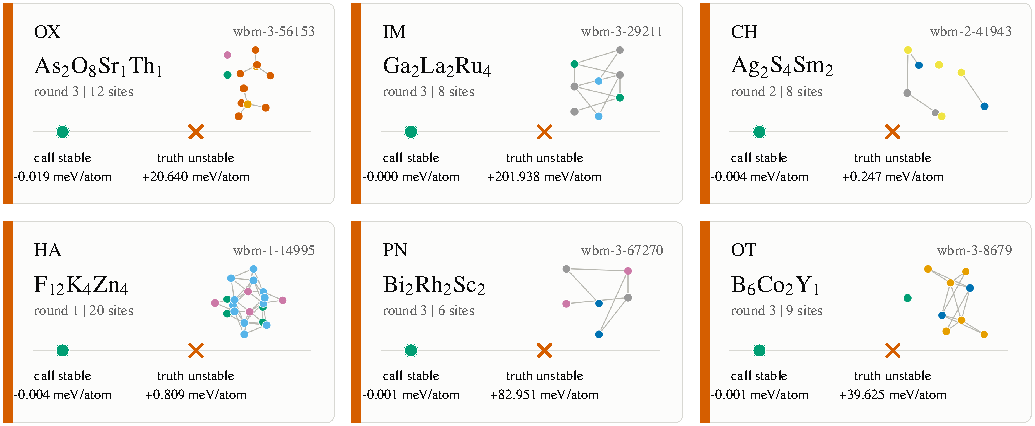
\includegraphics[width=\textwidth]{candidate_cases.pdf}
  \caption{Illustrative frozen object-level candidates at the stable-call boundary, one per
  anion-priority chemistry stratum for CHGNet on the MP-generation WBM set. Each card identifies
  the real WBM candidate and composition, then contrasts the reconstructed predicted hull call
  with the corrected WBM hull label. The six cards are selected deterministically within stratum
  among false-positive stable calls by minimum absolute predicted hull distance; they are boundary
  examples, not a representative sample or performance estimate. Each card pairs the initial WBM
  structure with its composition, predicted hull call, and corrected WBM reference label. Chemistry codes are
  OX/oxide, IM/intermetallic, CH/chalcogenide, HA/halide, PN/pnictide, and OT/other.}
  \label{fig:candidatecases}
\end{figure}

\begin{figure}[t]
  \centering
  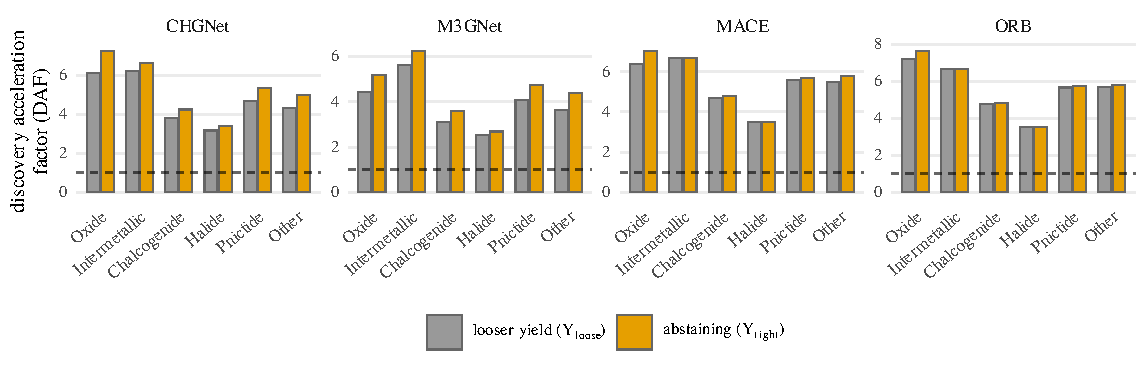
\includegraphics[width=\textwidth]{F1_daf_coverage.pdf}
  \caption{Matched-yield DAF at the looser ($Y_{\mathrm{loose}}$) and tighter
  ($Y_{\mathrm{tight}}$, abstaining) yield budgets, per anion-class stratum and per model.
  Oxides show the largest DAF lift from abstention; halides and intermetallics the smallest.
  The dashed reference at DAF\,$=1$ in each panel marks the no-acceleration baseline (surfaced
  precision equal to stratum base rate; abstention buys no precision gain). All four panels use
  the same vertical scale, enabling direct comparison across models. Chemistry codes are
  OX/oxide, IM/intermetallic, CH/chalcogenide, HA/halide, PN/pnictide, and OT/other.}
  \label{fig:f1}
\end{figure}

\subsection{The stratum $\times$ coverage interaction fires, oxide-anchored and positive}

Figure~\ref{fig:f2} renders the matched-yield interaction $\mathrm{gain}_A - \mathrm{gain}_B$
for every (model, stratum-pair) cell; outlined cells have a 95\,\% bootstrap CI excluding
zero. Of the 60 cells, 48 exclude zero under an i.i.d.\ bootstrap, and all four models
contribute (CHGNet 13/15, MACE 13/15, M3GNet 11/15, ORB 11/15). Because WBM is generated by
elemental substitution into shared prototypes, structures sharing a parent prototype are
correlated; we therefore recompute the CIs with a prototype-blocked bootstrap that
resamples structural-prototype clusters within each stratum (block $=$ WBM AFLOW
prototype). Under blocking 45 of 60 cells still exclude zero (the shuffle-null stays
$0/60$), and we adopt this as the primary count. The three cells that drop out are all
borderline intermetallic pairs whose i.i.d.\ CI already grazed zero (M3GNet
oxide--intermetallic and intermetallic--chalcogenide, ORB intermetallic--pnictide); no
oxide-vs-halide or strong oxide cell is affected. The firing cells are dominated by
oxide-anchored pairs: 18 of 20 oxide-containing cells fire under i.i.d.\ resampling and 17 of
20 under blocking, with oxide as the higher-benefit stratum --- a direction first observed at
Stage-1 and documented, not registered ex ante, in
the Stage-2 analysis record; the general
stratum-interaction hypothesis and kill criterion were committed ex ante in
a dated pre-analysis design memo. The largest interaction is CHGNet's
oxide-vs-halide pair at $+0.90$ (prototype-blocked 95\,\% CI $[0.74, 1.04]$; i.i.d.\ CI
$[0.77, 1.04]$); the median absolute interaction across all 60 cells is $0.19$. These counts
survive formal multiplicity control
with two-sided bootstrap sign
$p$-values per cell, Benjamini--Hochberg at $q=0.05$ retains 46/60 cells (shuffle-null:
0/60), and a higher-resolution pass ($10^4$ bootstrap draws, same seed and machinery)
retains 40/60 under the stricter family-wise Holm--Bonferroni procedure at
$\alpha = 0.05$; the headline CHGNet oxide-vs-halide cell has Holm-adjusted
$p = 0.012$. The interaction is thus empirically oxide-anchored; the next subsection dissects
its mechanism directly from the predictions and finds it is driven by error-headroom and
base-rate normalization, not by hull-margin confidence being intrinsically sharper in oxide
chemistry.

\begin{figure}[t]
  \centering
  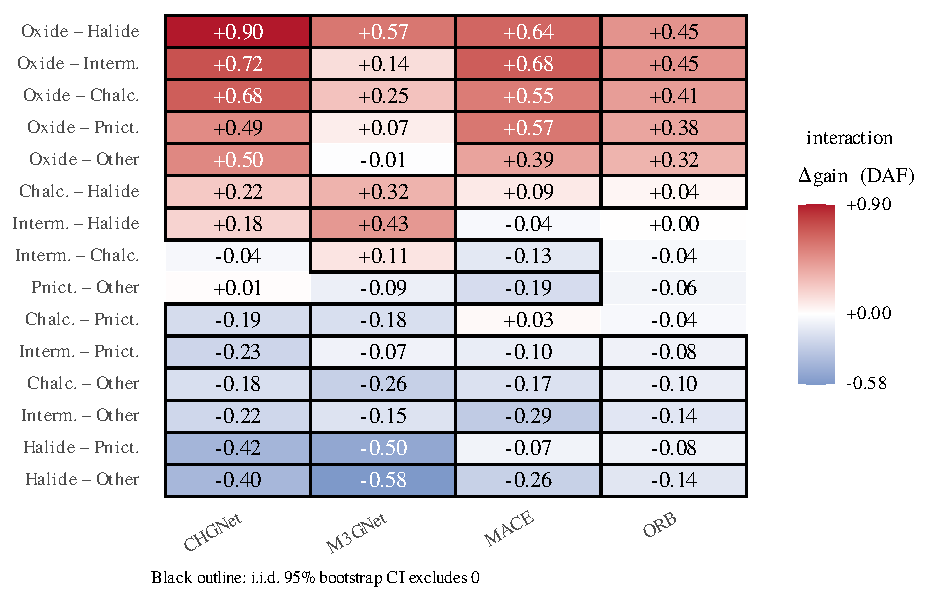
\includegraphics[width=0.82\textwidth]{F2_interaction_heatmap.pdf}
  \caption{Stratum $\times$ coverage interaction (median $\mathrm{gain}_A - \mathrm{gain}_B$)
  per model and stratum pair. Black outlines mark the 48/60 cells whose i.i.d.-bootstrap
  95\,\% CI excludes zero; the separate prototype-blocked sensitivity analysis retains 45/60
  cells (the primary count --- Results). The diverging fill scale spans the full observed
  interaction range and is centered at zero. Oxide-anchored pairs are positive across models.}
  \label{fig:f2}
\end{figure}

\subsection{Mechanism: error headroom and base-rate normalization, not sharper confidence}

To test the naive reading --- that hull-margin confidence simply discriminates oxide errors
better --- we compute three post-hoc descriptive diagnostics per stratum directly from the
cached predictions (averaged over the four UIPs in Table~\ref{tab:mechanism}; full per-model
values in the reproduction archive). Two findings reframe the mechanism. First, oxides carry by
far the largest UIP formation-energy error --- RMSE $0.62$\,eV/atom versus $\sim\!0.09$ for every
other stratum --- so a large share of the structures a UIP calls stable in oxides are false
positives (called-stable precision $0.75$), leaving room for abstention to raise precision.
Second, and against the naive reading, the within-stratum rank-informativeness of the
confidence signal (AUROC of $|\hat{e}_{\mathrm{hull}}|$ separating truly-stable from
false-positive called-stable structures) is if anything the lowest of the six strata in
oxides ($0.69$ versus $0.75$--$0.78$ elsewhere): confidence does not discriminate oxide errors
better per structure. The oxide anchoring instead arises from two compounding factors --- the
large error creates the false-positive headroom, and because DAF normalizes precision by the
stratum stable base rate, which is lowest in oxides ($12.4\,\%$ versus $27.8\,\%$ for halides),
an equal precision gain from abstention becomes a larger DAF gain. These two amplifications
should be read separately, because DAF folds a genuine precision-recovery advantage together
with the $1/\text{base-rate}$ factor. In precision-point units the CHGNet oxide-vs-halide
abstention advantage is $+7.7$ points (oxide called-stable precision lifts $+14.3$ points under
abstention, halide only $+6.6$); the headline $+0.90$ DAF interaction is that $2.2\times$
precision-recovery advantage further multiplied by DAF's $2.2\times$ base-rate denominator
(halide $27.8\,\%$ / oxide $12.4\,\%$), so the $\sim\!4.9\times$ cross-stratum DAF-gain ratio
is roughly half genuine precision headroom and half base-rate normalization. We report the
precision-unit interaction alongside DAF throughout so the base-rate amplification is transparent.
The effect is
real and reproducible --- it is exactly what the shuffle-null, LOEO, round, and
alternative-stratification controls certify --- but it is an interaction between error-driven
headroom and base-rate-normalized reporting, not evidence that a UIP is more trustworthy when
confident in oxide chemistry specifically.

\begin{table}[t]
  \centering
  \caption{Post-hoc descriptive per-stratum mechanism diagnostics, averaged over the four UIPs.
  Oxides combine the largest formation-energy error and the lowest stable base rate with ---
  against the naive reading --- the lowest confidence-rank AUROC. Base rate is the
  stratum stable fraction; RMSE is the formation-energy error; called-stable precision is the
  true-stable fraction among structures called stable; AUROC is the rank separation of
  $|\hat{e}_{\mathrm{hull}}|$ for truly-stable versus false-positive called-stable structures.}
  \label{tab:mechanism}
  \begin{tabular}{lcccc}
    \toprule
    Stratum & Base rate & RMSE (eV/atom) & Called-stable prec. & Conf.\ AUROC \\
    \midrule
    Oxide          & 0.124 & 0.625 & 0.747 & 0.695 \\
    Intermetallic  & 0.142 & 0.091 & 0.631 & 0.756 \\
    Chalcogenide   & 0.205 & 0.088 & 0.725 & 0.766 \\
    Halide         & 0.278 & 0.090 & 0.752 & 0.756 \\
    Pnictide       & 0.171 & 0.097 & 0.680 & 0.775 \\
    Other          & 0.167 & 0.097 & 0.641 & 0.772 \\
    \bottomrule
  \end{tabular}
\end{table}

\paragraph{What the interaction buys a practitioner.} Concretely, for CHGNet --- the strongest
firer of the four UIPs, so this is a best-case illustration rather than a typical one --- the
$+0.90$ oxide-versus-halide interaction converts as follows, on the \emph{pooled} evaluation
(post-hoc descriptive, from the frozen matched-yield DAF; this pooled framing is the one that
does not transfer temporally, per Threats to validity). Of the $2{,}696$ structures CHGNet
calls stable in oxides, keeping only the
$1{,}348$ most confident by $|\hat{e}_{\mathrm{hull}}|$ raises true-stable precision from
$75.8\,\%$ to $90.1\,\%$ (DAF $6.1 \to 7.2$). A practitioner with a fixed budget of $1{,}348$
DFT relaxations therefore wastes $\sim\!134$ of them on false positives by spending it on the
confident half, versus $\sim\!326$ by spending it on a same-size random draw from all
called-stable oxides --- roughly $190$ fewer wasted relaxations. The identical abstention on
halides moves precision only $88.2\,\% \to 94.8\,\%$ (DAF $3.2 \to 3.4$; halide base DAF $3.01$,
cf.\ the provenance footnote), saving $\sim\!90$ relaxations --- about half the oxide payoff,
which is the concrete practitioner form of the interaction.

\subsection{The interaction is robust to held-out chemistry and acquisition round}

Figure~\ref{fig:f3} reports the fraction of firing cells under each robustness split.
Under LOEO, all 12 held-out-element splits remain majority-firing (12/12), pooling to
548/700 cells (538/700 under the prototype-blocked bootstrap, all 12 splits still
majority-firing); crucially, dropping oxygen --- which empties the entire oxide stratum and
leaves only 5 strata (40 cells) --- still fires 37/40 (36/40 blocked), so the effect is
not carried by
oxides alone, and no single cation or anion-former split falls below 39/60. Under the
WBM-round gate, 3 of 5 rounds are majority-firing (rounds 1--3: 43/34/43 of 60), pooling to
157/300 cells (151/300 blocked, the same 3 rounds majority-firing). Rounds 4 and 5 fall below majority (26 and 11 of 60); these are the two
smallest rounds (40k and 23k rows), so the shortfall is a per-model power effect under tiny
matched-yield budgets, not a temporal sign flip --- the oxide-highest direction is preserved
even where the CIs widen. The majority-of-splits / majority-of-rounds success criterion,
documented alongside the Stage-2 results themselves rather than registered before Stage-1,
is met on both axes.

\begin{figure}[t]
  \centering
  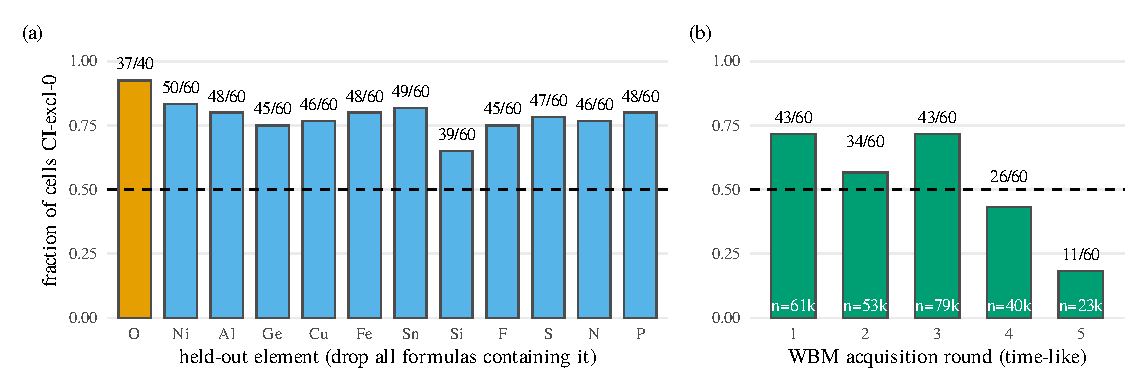
\includegraphics[width=\textwidth]{F3_robustness_panel.pdf}
  \caption{Fraction of (model $\times$ stratum-pair) cells whose 95\,\% CI excludes zero,
  per robustness split. (a) leave-one-element-out (12/12 splits majority-firing); (b)
  WBM round (3/5 rounds majority-firing). Cell counts annotated; dashed line is the majority
  threshold. In panel (a), the O bar is coloured to flag the 5-stratum / 40-cell case
  (dropping O empties the oxide stratum entirely; the 37/40 count is out of 40, not 60).
  In panel (b), the $n{=}X$k sub-bar labels give the row count per WBM acquisition round
  (rounds 1--5 carry 61k, 53k, 79k, 40k, 23k rows respectively).}
  \label{fig:f3}
\end{figure}

The held-out-UIP hierarchical bootstrap (Figure~\ref{fig:e2forest}) re-estimates the
population-average oxide$|$halide interaction under architecture-family blocking
(32 included UIPs across 12 families, orb\_v2\_omat duplicate excluded; $10^4$
bootstrap replicates, family as the cluster unit); the family-blocked 95\,\% CI
is $[+0.604,\,+0.848]$ with population median $+0.721$, and no architecture family
falls below the CI lower bound. The leave-one-family-out worst case (dropping
dpa3) still leaves a population mean of $+0.680$, so the headline interaction
generalises across the audited UIP population and is not carried by a single
architecture or shared training corpus. This addresses the model-pseudoreplication
objection that row-level prototype-blocked CIs do not speak to directly.

\begin{figure}[!htbp]
  \centering
  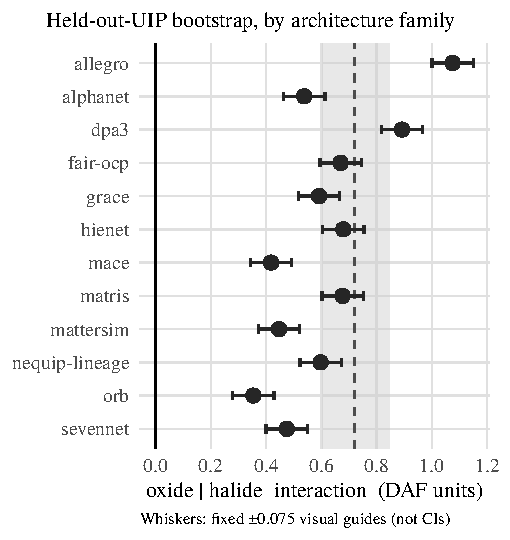
\includegraphics[width=0.62\textwidth]{e2_family_blocked_ci.pdf}
  \caption{Held-out-UIP hierarchical bootstrap, per architecture family. Each point
  is the family-blocked mean oxide$|$halide interaction for the indicated family. Uniform
  $\pm0.075$ whiskers are fixed visual references for comparing family means; they are not
  per-family confidence intervals. The gray band is the population 95\,\% CI
  $[+0.604,\,+0.848]$; the dashed line is the population median $+0.721$. No family's mean
  falls below the CI lower bound.}
  % script:  figures-source/integration_2026-07-21/e2_family_blocked_ci.R (R + Cairo PDF, TeX Gyre Termes serif, Type 1C embedded)
  % contract: 32 included UIPs, 12 architecture families, orb_v2_omat excluded
  \label{fig:e2forest}
\end{figure}

\subsection{The shuffle-null is clean everywhere}

Figure~\ref{fig:f4} contrasts the magnitude of the real interaction with the
confidence-shuffled interaction, per gate. Permuting confidence within each stratum's
called-stable set collapses the signal to a tight band around zero, and no shuffled
cell's CI excludes zero in any gate: 0/60 at Stage-1, 0/700 under LOEO, and 0/300 across
rounds. The largest shuffled Stage-1 interaction is $0.0047$ in absolute value, two orders
of magnitude below the real median. The interaction is therefore a property of the
confidence ordering, exactly what a genuine abstention effect requires.

\begin{figure}[t]
  \centering
  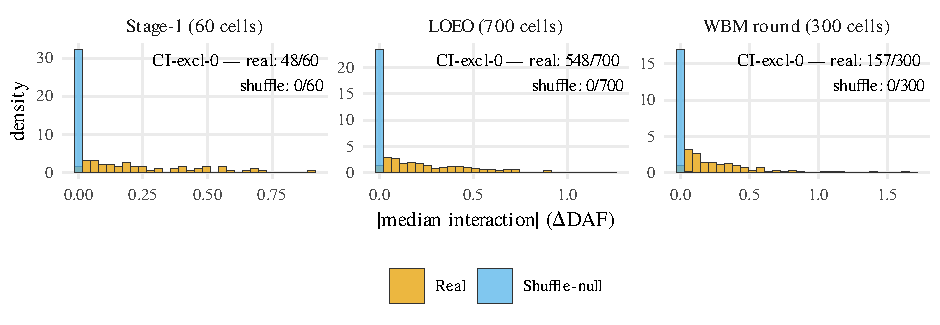
\includegraphics[width=\textwidth]{F4_shuffle_null.pdf}
  \caption{Real vs.\ within-stratum confidence-shuffled $|$interaction$|$ per gate. Real
  CIs exclude zero in 48/60 (Stage-1), 548/700 (LOEO), and 157/300 (WBM round) cells; the
  shuffled CIs exclude zero in 0/60, 0/700, and 0/300 cells respectively --- the
  shuffle-null collapses to zero in every gate.}
  \label{fig:f4}
\end{figure}

\subsection{Committee-variance abstention reproduces the interaction; native-Gaussian
coverage is optimistic in every chemistry}

Two further analyses probe whether the oxide-anchored abstention benefit is a quirk of the
particular confidence source. First, we replace each UIP's single-model
$|\hat{e}_{\mathrm{hull}}|$ with a \emph{committee-variance} signal: confidence
$=-\mathrm{std}$ of the four UIPs' reconstructed predicted hull distances, with the consensus
stable call taken as the committee-mean hull below zero, holding the matched-yield control
identical ($Y_{\mathrm{tight}} = 1422$, $Y_{\mathrm{loose}} = 2844$).
Figure~\ref{fig:f5}(a) shows the committee-variance abstention benefit is again concentrated
in oxides (matched-yield DAF gain median $+0.563$) and small elsewhere ($\le +0.10$; halide
$-0.014$). Of the 15 stratum-pair interactions, 7 have a 95\,\% bootstrap CI excluding zero
(Figure~\ref{fig:f5}(b)): all five oxide-anchored pairs positive (oxide-vs-halide $+0.574$,
CI $[0.463, 0.687]$) plus chalcogenide-vs-halide ($+0.115$, CI $[0.044, 0.183]$), with one
negative (halide-vs-pnictide $-0.114$, CI $[-0.211, -0.019]$), while the within-stratum
confidence shuffle fires 0/15. The committee's dominant interaction sign is positive,
matching the single-model reference, and it agrees in sign on all 7 jointly-significant
pairs, yet it fires far fewer pairs than the single-model consensus --- so it is a genuinely
distinct re-derivation of the effect, not a relabelling of one model. One limitation qualifies
this as \emph{corroboration} rather than independent confirmation: the committee is built from the
same four UIPs' predictions, so if those models share a correlated oxide error (plausibly through
the common MP2020-corrected labels they are trained and scored against; see Discussion), the
committee-variance signal inherits that oxide false-positive richness rather than
independently confirming it. It re-derives the interaction from a different \emph{functional} of
the same predictions, not from independent models (robustness gate verdict
PASS-BOTH; Table~\ref{tab:signalcompare}).

\begin{figure}[t]
  \centering
  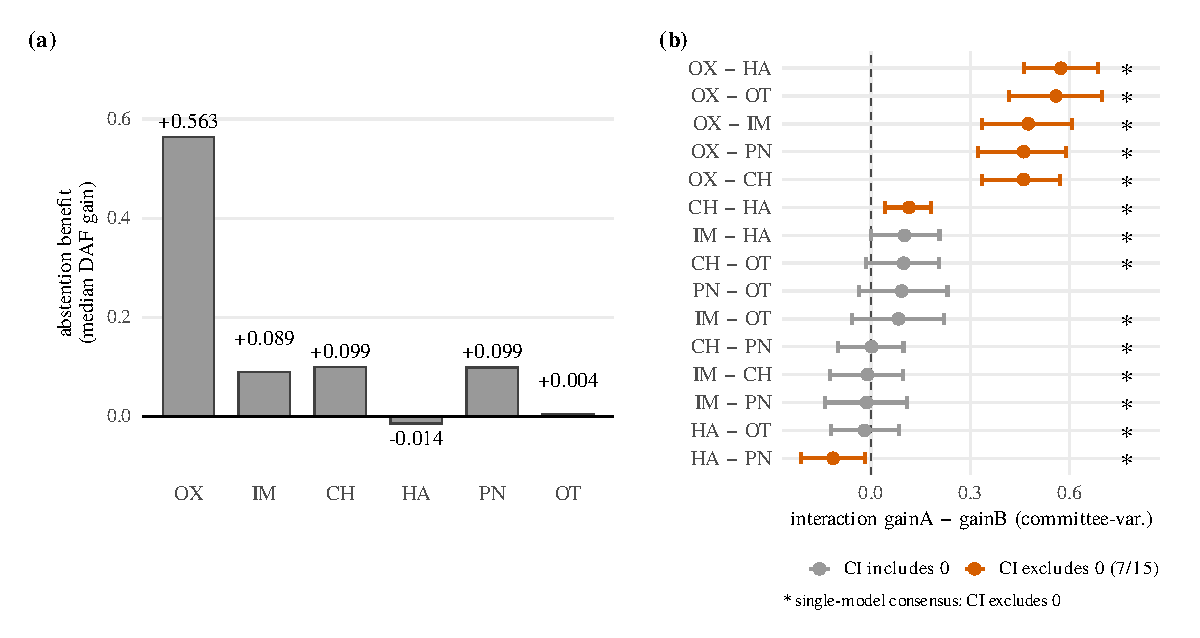
\includegraphics[width=\textwidth]{F5_committee_variance.pdf}
  \caption{Committee-variance abstention vs.\ the single-model signal. (a) Matched-yield DAF
  gain (median) per anion stratum using the committee-variance signal; the benefit
  concentrates in oxides, mirroring the single-model pattern. (b) The 15 stratum-pair
  committee-variance interactions ($\mathrm{gain}_A - \mathrm{gain}_B$, median with 95\,\%
  bootstrap CI); orange marks the 7 pairs whose committee CI excludes zero. A right-gutter
  asterisk means that the single-model consensus also excludes zero for that pair; it does not
  encode the committee CI. The committee is sparser (7/15) but sign-consistent; the
  confidence-shuffle collapses to 0/15. Chemistry codes are OX/oxide, IM/intermetallic,
  CH/chalcogenide, HA/halide, PN/pnictide, and OT/other.}
  \label{fig:f5}
\end{figure}

\begin{table}[t]
  \centering
  \caption{Abstention-signal comparison: the free single-model hull margin
  $|\hat{e}_{\mathrm{hull}}|$ vs.\ a four-UIP committee-variance signal, both under the
  identical matched-yield DAF control. Denominators differ because the committee collapses
  the model axis: single-model interaction cells are counted per (model $\times$
  stratum-pair) $=60$, committee interactions per stratum-pair $=15$. Both counts here use
  the i.i.d.\ bootstrap for an apples-to-apples comparison; the single-model primary count
  under the prototype-blocked bootstrap is 45/60 (Results).}
  \label{tab:signalcompare}
  \begin{tabular}{lcc}
    \toprule
    & Single-model $|\hat{e}_{\mathrm{hull}}|$ & Committee variance \\
    \midrule
    Confidence signal              & $|\hat{e}_{\mathrm{hull}}|$ per UIP & $-\mathrm{std}$ over 4 UIP hulls \\
    Stable call                    & predicted hull $<0$                & committee-mean hull $<0$ \\
    Matched-yield budget ($Y_{\mathrm{tight}}/Y_{\mathrm{loose}}$) & per model & $1422 / 2844$ \\
    Interaction cells CI-exclude-0 & 48/60                              & 7/15 \\
    Shuffle-null cells CI-exclude-0 & 0/60                              & 0/15 \\
    Dominant interaction sign      & $+$ (oxide-anchored)               & $+$ (oxide-anchored) \\
    Sign agreement, jointly-sig.\ pairs & ---                           & 7/7 \\
    Robustness gate verdict        & ---                                & PASS-BOTH \\
    \bottomrule
  \end{tabular}
\end{table}

Second, we ask whether a zero-free-parameter probabilistic reading of the same margin is
well-calibrated within each chemistry. Using the native Gaussian
$p_{\mathrm{stable}} = \Phi(-\hat{e}_{\mathrm{hull}}/\sigma)$, with $\sigma$ the
calibration-half RMSE of the formation-energy error, we measure the per-anion-family
conditional-coverage gap (mean $p_{\mathrm{native}}$ minus the empirical stable rate) on the
held-out test half. Every gap is positive and CI-excludes-zero for every UIP
(Table~\ref{tab:sscs}): the native Gaussian over-predicts stability in every family. The
worst-slab gap (SSCS $= \max_s |\mathrm{gap}_s|$) ranges from ORB's $0.077$ (best calibrated)
to MACE's $0.322$ (worst, driven by its inflated $\sigma = 0.977$, which pushes $p$ toward
$0.5$ everywhere), with a cross-model mean of $0.197$. Two distinct chemistry dependences must
not be conflated here. Calibration miscalibration (whether $p_{\mathrm{stable}}$ matches the
empirical stable rate) and abstention headroom (whether ranking by $|\hat{e}_{\mathrm{hull}}|$
can lift precision) are different properties: the native Gaussian is optimistic in every family,
but the stratum where it fails hardest is intermetallics for three of the four
UIPs (CHGNet, M3GNet, ORB; Table~\ref{tab:sscs}), not oxides, and only MACE has its worst
calibration gap in oxides. The abstention benefit, by contrast, is oxide-anchored for all four
models. The two axes therefore co-locate in oxides only for MACE; in general the chemistry a
UIP is least calibrated on is not the chemistry where abstention pays most.

\begin{table}[t]
  \centering
  \caption{Native-Gaussian ($p_{\mathrm{stable}} = \Phi(-\hat{e}_{\mathrm{hull}}/\sigma)$,
  zero free parameters) per-anion-family conditional-coverage gap (mean $p_{\mathrm{native}}$
  minus empirical stable rate) on the test half, per UIP. Every gap is positive and its
  95\,\% bootstrap CI excludes zero, so the native Gaussian over-predicts stability in every
  family for every model. SSCS is the worst-slab $\max_s |\mathrm{gap}_s|$.}
  \label{tab:sscs}
  \begin{tabular}{lcccccccc}
    \toprule
    UIP & $\sigma_{\mathrm{cal}}$ & Oxide & Interm. & Chalc. & Halide & Pnict. & Other & SSCS (worst) \\
    \midrule
    CHGNet & 0.102 & 0.109 & 0.177 & 0.139 & 0.126 & 0.148 & 0.161 & 0.177 (interm.) \\
    M3GNet & 0.117 & 0.172 & 0.214 & 0.200 & 0.177 & 0.195 & 0.207 & 0.214 (interm.) \\
    MACE   & 0.977 & 0.322 & 0.315 & 0.246 & 0.199 & 0.277 & 0.287 & 0.322 (oxide) \\
    ORB    & 0.081 & 0.074 & 0.077 & 0.048 & 0.055 & 0.038 & 0.052 & 0.077 (interm.) \\
    \midrule
    \multicolumn{8}{l}{Mean SSCS over models} & 0.197 \\
    \bottomrule
  \end{tabular}
\end{table}

\subsection{Roster-wide universality (32 modern UIPs)}
\label{sec:roster-universality}
\paragraph{Inclusion rule and the 32-UIP sample.} Following the pre-specified inclusion rule
($\ge\!50$ called-stable structures per stratum and $\ge\!99\%$ WBM coverage, which keeps the
common-yield budget non-degenerate), $32$ modern UIPs qualify ($16$ MP-generation, $16$
OMat-generation, after dropping the non-independent duplicate of the MP-generation ``orb'' anchor).
The per-model oxide-vs-halide matched-yield interaction is positive with a prototype-blocked
95\,\% CI excluding zero for all $32$ ($16/16$ MP-generation, $16/16$ OMat-generation);
oxide is the single highest-benefit stratum in $29/32$ (the three exceptions are
MP-generation models whose arg-max is the residual ``other'' stratum, not a reversal);
per-model interactions range from $+0.31$ to $+1.31$ (Table~\ref{tab:roster}). The
pre-specified hypothesis that the newer OMat generation would dissolve or reverse the anchoring
is not supported: a model-level permutation test on the generation label gives $p = 0.68$
(observed MP$-$OMat gap in mean interaction $-0.037$, 95\,\% CI $[-0.21, 0.13]$; $n_{\mathrm{MP}} = 16$,
$n_{\mathrm{OMat}} = 16$). We read this as no detectable generational difference in the oxide anchor:
the CI is wide relative to the observed gap and the analysis is underpowered (at $n=16$ per arm) to
exclude a moderate-magnitude generational shift, so ``generation-independent'' should be read as
an honest null within this roster's power, not as a demonstrated invariance.

\paragraph{Classical baselines and multiplicity.} The seven 2020-era classical baselines
(CGCNN, CGCNN+P, MEGNet, Wrenformer, Voronoi-RF, ALIGNN, BOWSR-MEGNet; all MP-trained) are by
contrast weak and mixed --- five carry a positive CI-excluding oxide-vs-halide interaction but
oxide is the arg-max stratum for only two, and Voronoi-RF reverses it ($-0.12$, CI $[-0.22, -0.02]$)
--- so the effect is specific to modern universal potentials, not shared by every ML
formation-energy model. Over the full included-UIP interaction family ($32 \times 15 = 480$
cells) $378$ CI-exclude zero and $369$ survive Benjamini--Hochberg FDR~\citep{benjamini1995fdr}
at $q = 0.05$; the oxide-vs-halide subfamily is $32/32$ under both, with a clean within-stratum
confidence-shuffle null ($0/480$). The Holm--Bonferroni family-wise procedure~\citep{holm1979}
survives $0/480$ (and $0/32$ on the oxide-halide subfamily) at $\alpha = 0.05$: this is a
bootstrap-resolution limit, not evidence against the effect --- the minimum achievable two-sided
bootstrap $p$ at $n_{\mathrm{boot}} = 1000$ is $\approx\!0.002$, and Holm's family-wise correction
over $480$ (or $32$) cells demands $p < 0.05/480 \approx 1.0\times10^{-4}$ (or
$0.05/32 \approx 1.6\times10^{-3}$), both below the achievable floor; the BH-FDR and raw-CI readings above are
the informative ones here, mirroring the treatment of the equivalent Stage-1 Holm result.

\paragraph{Two published files with non-physical MAE, retained with disclosure.} Two MP-generation
files in the published Matbench Discovery prediction release --- GRACE-2L-MPtrj and SevenNet-0 --- contain a handful of
catastrophic-outlier prediction rows ($13$ and $1$ of $256{,}963$, with $|\hat{e}_{\mathrm{form}}|$
up to $10^{22}$ and $10^{33}$\,eV/atom) that make their naive mean absolute error
non-physical ($5\times10^{16}$ and $10^{28}$\,eV/atom); trimming those rows restores physical MAEs
of $0.057$ and $0.046$\,eV/atom. Because the analysis ranks and thresholds predictions rather than
averaging them, these rows do not affect the result: removing them shifts each oxide-vs-halide
interaction by $\le\!0.013$ (well inside its $\sim\!0.3$-wide CI) and leaves the arg-max stratum
and CI-exclusion unchanged, so both models are retained among the $32$ with this disclosure rather
than silently trimmed.

\begin{table}[t]
  \centering
  \small
  \caption{Roster-wide oxide-vs-halide matched-yield abstention interaction $I$ (prototype-blocked
  95\,\% CI) for all $32$ included modern UIPs, by training generation (models are Matbench
  Discovery leaderboard identifiers; the published Orb-v2
  OMat file is excluded here as a non-independent duplicate of the MP-generation ``orb'' anchor,
  text). $I>0$ with CI excluding zero for all $32$; oxide is the highest-benefit stratum in $29$.
  GRACE-2L-MPtrj and SevenNet-0 carry non-physical published MAE from a few outlier rows that do
  not affect this rank-based interaction (text).}
  \label{tab:roster}
  \begin{tabular}{lcc@{\hskip 1.4em}lcc}
    \toprule
    \multicolumn{3}{c}{MP generation ($n=16$)} & \multicolumn{3}{c}{OMat generation ($n=16$)} \\
    \cmidrule(lr){1-3}\cmidrule(lr){4-6}
    model & $I$ & 95\,\% CI & model & $I$ & 95\,\% CI \\
    \midrule
    eqv2\_s\_mp & $+1.16$ & $[1.02,1.29]$ & allegro\_oam & $+1.31$ & $[1.19,1.44]$ \\
    matris\_mptrj & $+1.01$ & $[0.88,1.13]$ & dpa31\_ft & $+1.13$ & $[1.00,1.25]$ \\
    dpa3\_v2\_mptrj & $+0.99$ & $[0.86,1.13]$ & dpa3\_v2\_openlam & $+0.98$ & $[0.86,1.11]$ \\
    allegro\_mp & $+0.95$ & $[0.80,1.11]$ & grace\_1l\_oam & $+0.91$ & $[0.77,1.04]$ \\
    grace\_2l\_mptrj & $+0.91$ & $[0.76,1.06]$ & eqv2\_m\_omat & $+0.90$ & $[0.77,1.03]$ \\
    mattersim & $+0.83$ & $[0.71,0.94]$ & dpa3\_v1\_openlam & $+0.83$ & $[0.71,0.96]$ \\
    dpa3\_v1\_mptrj & $+0.83$ & $[0.70,0.95]$ & alphanet\_oma & $+0.70$ & $[0.58,0.82]$ \\
    hienet & $+0.74$ & $[0.60,0.87]$ & esen\_oam & $+0.70$ & $[0.58,0.81]$ \\
    nequip\_mp & $+0.59$ & $[0.45,0.73]$ & nequip\_oam\_xl & $+0.67$ & $[0.55,0.77]$ \\
    matris\_10m\_mp & $+0.58$ & $[0.47,0.69]$ & orb\_v3 & $+0.64$ & $[0.52,0.76]$ \\
    eqnorm\_mptrj & $+0.50$ & $[0.37,0.63]$ & mace\_mpa & $+0.62$ & $[0.48,0.75]$ \\
    alphanet\_mp & $+0.49$ & $[0.37,0.61]$ & grace\_3l\_oam & $+0.57$ & $[0.45,0.67]$ \\
    sevennet\_0 & $+0.48$ & $[0.34,0.61]$ & grace\_2l\_oam & $+0.55$ & $[0.44,0.68]$ \\
    nequix\_mp & $+0.42$ & $[0.29,0.57]$ & nequip\_oam & $+0.54$ & $[0.42,0.64]$ \\
    sevennet\_l3i5 & $+0.41$ & $[0.27,0.55]$ & matris\_oam & $+0.50$ & $[0.40,0.61]$ \\
    esen\_mp & $+0.38$ & $[0.25,0.52]$ & grace\_2l\_oam\_l & $+0.31$ & $[0.19,0.42]$ \\
    \bottomrule
  \end{tabular}
\end{table}

\section{Discussion}

\subsection{Interpretation of the oxide-anchored interaction}

\paragraph{What the result means.} The value of selective abstention in UIP stability
screening is not uniform across chemistry, and where it is largest tracks where the reference
data is least trustworthy. At a surfaced-candidate budget held identical across
anion classes, abstaining on low-confidence calls accelerates discovery substantially more
in oxides than in halides or intermetallics --- but the load-bearing quantity is a genuine
precision advantage, not the base-rate-amplified DAF headline. Decomposed (Results,
Table~\ref{tab:mechanism}), the CHGNet oxide-vs-halide abstention gain is $+7.7$ precision
points; DAF's normalization by the low oxide base rate then amplifies that to the $+0.90$ DAF
figure, so roughly half the DAF headline is a reporting denominator and only the precision-point
interaction should be read as the effect size. The precision advantage itself does not arise
because hull-margin confidence is intrinsically sharper in oxide chemistry --- its within-oxide
rank-AUROC is if anything the lowest of the six strata --- but because oxide formation energies
are where UIP predictions disagree most with the (least trustworthy) MP2020 labels, by a wide
margin (RMSE $\sim\!0.6$ versus $\sim\!0.09$\,eV/atom elsewhere), so the largest share of oxide
stable-calls are false positives and confidence-based abstention has the most precision to
recover. Both compounding factors --- the false-positive headroom and the base-rate denominator
--- therefore point at the same place: the chemistry where the DFT reference is weakest. That is
why we read the interaction as a diagnostic of reference-data trustworthiness rather than a
chemistry-specific abstention policy. Intermetallics, by
contrast, contribute few CI-firing cells for MACE and ORB, whose intermetallic gain is
statistically indistinguishable from zero.

\paragraph{The oxide anchoring is not manufactured by WBM's construction.} A natural worry is
that the effect is an artifact of how the WBM test set is built --- elemental substitution into
known prototypes~\citep{wang2021} --- rather than a property of UIP reliability. Three features
of the analysis rule this out. First, the interaction is measured in DAF (precision normalized
by each stratum's own stable base rate) under a matched-yield control that fixes the same
absolute number of surfaced candidates in every stratum, so neither the abundance of
oxides in WBM (they are $\sim\!10\,\%$ of the joined set, not a dominant class) nor their base
rate can mechanically inflate the oxide gain --- both quantities are divided or held out.
Second, the driving quantity is the UIPs' formation-energy error, which is $\sim\!7\times$ larger
in oxides (Table~\ref{tab:mechanism}) and appears at near-identical magnitude across four
independently trained architectures; a sampling artifact of WBM would not reproduce the same
oxide-error signature across unrelated models, whereas a genuine transferability gap on oxide
chemistry would. Third, the effect survives controls that a construction artifact should not:
dropping oxygen entirely still fires the interaction ($37/40$ cells), the metal-fraction and
electronegativity stratifications --- which never reference oxide membership --- reproduce it,
and the time-like WBM-round splits preserve its direction. The oxide anchoring therefore reflects
where UIPs are least accurate, not how WBM was assembled.

\paragraph{Why UIP--label disagreement is largest in oxides --- and why the oxide labels are
least trustworthy there.} The diagnostics establish that the disagreement between a UIP's
predicted formation energy and its MP2020-corrected training label is largest in oxides
(Table~\ref{tab:mechanism}). We are careful about the level of this statement. The UIPs are
trained on the already-MP2020-corrected labels~\citep{deng2023,wang2021mp2020}, so their
residual is a model fitting error on corrected targets, not a leakage of the semilocal-DFT
(GGA) error into the prediction --- that GGA error lives in the labels and is corrected before the
model ever sees it. Two documented properties of universal potentials make oxides the hardest
chemistry to fit: a systematic potential-energy-surface softening / energy underprediction shared
across uMLIP architectures~\citep{deng2025softening}, and a per-chemistry error concentration in
oxide and transition-metal chemistry reported in independent
assessments~\citep{yu2024assessment}. The MP2020 corrections are themselves
composition- and oxidation-state-dependent step functions~\citep{wang2021mp2020} that a smooth
interatomic potential is ill-suited to reproduce, which plausibly amplifies the oxide fitting gap
(the anomalously large oxide formation-energy RMSE in Table~\ref{tab:mechanism}, several times the
models' aggregate error, is consistent with such a hard-to-fit seam and is not separately
isolated here). Compounding this, the oxide labels are also the least reliable slice of the
ground truth: correlated-$d$ transition-metal oxides require a Hubbard-$U$ treatment that the
PBE-based Materials Project reference does not consistently carry~\citep{wang2006oxidation,
jain2011formation}, and the very existence of the MP2020 anion/oxidation-state corrections is a
symptom that oxide DFT energetics carry uncorrected seams. Two things therefore co-locate in
oxides --- the chemistry a UIP fits worst, and the chemistry whose reference energies are least
trustworthy --- and our disagreement metric cannot separate them. The abstention benefit is
present in main-group oxides too (Table~\ref{tab:tmoxide}), so it is not carried by the
correlated-$d$ sub-family alone; but we do not claim to have isolated a single physical cause. The
demonstrated result remains the two-factor account of the abstention benefit above (error headroom
$\times$ base-rate normalization), now read as headroom in UIP--label disagreement rather
than in UIP error against a trusted truth.

\subsection{Robustness of the headline result}

\paragraph{The oxide benefit is not a transition-metal-oxide artifact.} Splitting the oxide
stratum into transition-metal oxides (formula containing a $d$-block metal; $17{,}369$ structures)
and main-group oxides ($7{,}651$) shows the matched-yield abstention benefit is present in
both sub-families for all four UIPs (Table~\ref{tab:tmoxide}): keeping the more-confident
half of each sub-family's called-stable structures gives a positive DAF gain in every
(model, sub-family) cell. Main-group oxides, which lack the transition-metal $d$-electron
localization seam, show a comparable benefit, so the effect is not carried by transition-metal
oxides alone --- consistent with the anion-level (oxygen) DFT correction being the broad driver of
the oxide error (post-hoc descriptive; full values in the reproduction archive).

\begin{table}[t]
  \centering
  \caption{Within-oxide split (post-hoc descriptive): matched-yield abstention detail for
  transition-metal oxides ($n=17{,}369$) versus main-group oxides ($n=7{,}651$), per UIP.
  $n$ called-stable is the sub-family's called-stable count at the loose budget; precision is
  the true-stable fraction among called-stable structures, full budget $\to$ confident half.
  DAF gain is positive in all eight cells.}
  \label{tab:tmoxide}
  \begin{tabular}{llccc}
    \toprule
    UIP & Sub-family & $n$ called-stable & Precision (full$\to$half) & DAF gain \\
    \midrule
    CHGNet & TM-oxide    & 1778 & $0.771\to0.917$ & $+1.24$ \\
           & Main-group  & 918  & $0.733\to0.867$ & $+0.97$ \\
    M3GNet & TM-oxide    & 2907 & $0.512\to0.579$ & $+0.56$ \\
           & Main-group  & 1292 & $0.632\to0.785$ & $+1.11$ \\
    MACE   & TM-oxide    & 2221 & $0.757\to0.825$ & $+0.58$ \\
           & Main-group  & 1047 & $0.860\to0.973$ & $+0.83$ \\
    ORB    & TM-oxide    & 2003 & $0.878\to0.950$ & $+0.61$ \\
           & Main-group  & 962  & $0.922\to0.938$ & $+0.11$ \\
    \bottomrule
  \end{tabular}
\end{table}

\paragraph{What DFT verification would and would not add.} The estimand throughout is
agreement with WBM's MP2020-compatible DFT ground truth~\citep{wang2021mp2020,riebesell2025}:
every stable call, abstention, and flip is scored against an already-computed DFT hull
distance, so the precision, DAF, and coverage numbers are DFT-referenced by construction.
Running new DFT on the flipped or abstained candidates would test the fidelity of the WBM
ground truth itself --- upstream of our contribution and shared by every Matbench Discovery
result --- not any claim made here, so we run none. One caveat bounds the oxide reading: the
audit inherits the labels' reliability, and the oxide labels are the benchmark's least
reliable slice (Sec.~\ref{sec:results}), so the finding is best read as ``UIP--label disagreement is
largest, and least trustworthy, in oxides,'' not as UIP error against a fully trusted truth.

\paragraph{Why this survives where the ``beats margin'' wedge did not.} The companion study
tested whether a learned or calibrated confidence signal (isotonic $p_{\mathrm{stable}}$,
cross-model disagreement) beats hull margin at matched coverage and matched stable-call
yield, and found that none did (0/12 cells): margin was undefeated, not shown insufficient. The
present result does not contradict that; it asks a different, orthogonal question --- whether
margin's own well-established abstention benefit is uniform across chemistry, and finds it is
not. Pooling oxides (large benefit) with intermetallics (no benefit) at matched yield washes
the average out, so the signal lives in the interaction across anion strata, not in a
main-effect claim about whether margin beats some other baseline, which is why it survives
the same common-absolute-yield control that companion study used. We carried that control
through genuine anion-class strata, leave-one-element-out, and WBM-round splits, and it survives
all of them with a clean shuffle-null.

\subsection{Relation to prior work and methodological precedent}

\paragraph{Relation to certified and ensemble-uncertainty approaches.} Two adjacent
literatures address confidence for UIPs, but neither reports a chemistry-conditioned value of
abstention. Proof-Carrying Materials~\citep{pcm2026} delivers a global, non-stratified
risk-of-failure model (AUC-ROC $0.938$) backed by formal safety certificates --- a
calibration/certification contribution, not a stratum $\times$ coverage DAF interaction, and
it reports no chemistry-conditioned abstention benefit. Multi-head-committee ensemble
uncertainty~\citep{beck2025} instead constructs a richer confidence signal (committee-of-heads
prediction standard deviation) and validates it via force-error correlation and
active-learning data efficiency; it neither uses the free $|\hat{e}_{\mathrm{hull}}|$ baseline
nor tests whether the value of any confidence signal for stability screening varies by
chemistry. Recent calibration-focused work on UIP uncertainty --- flexible post-hoc
calibration~\citep{ho2026flexcalib} and uncertainty quantification for \emph{misspecified}
potentials~\citep{perez2025uqmisspec} --- sharpens the confidence estimate itself but likewise
does not condition the value of abstention on chemistry. Closest in framing,
PROBE~\citep{probe2026} recasts UIP reliability as
\emph{selective classification} via a post-hoc probe on frozen representations, but does so at
the per-atom level during molecular dynamics rather than at the WBM stability decision, and
reports no chemistry-conditioned value of abstention. The present work is orthogonal to all
three: it is deliberately agnostic to the source
of the confidence signal --- the oxide-anchored interaction persists whether the signal is the
cheapest single-model $|\hat{e}_{\mathrm{hull}}|$ or a four-model committee variance
(Figure~\ref{fig:f5}, Table~\ref{tab:signalcompare}) --- and isolates a stratum-dependent
abstention benefit that neither the certification nor the ensemble-uncertainty literature
reports. In Digital Discovery, \citet{yu2026uaal} similarly probes the reliability limits of
uncertainty-aware screening --- there, uncertainty-guided active learning for lead-free halide
perovskites, where the confidence signal recurrently flags heavy $d$-electron halides as likely
functional-driven false positives. Our matched-yield audit occupies the same
reliability-of-screening lane at benchmark scale ($32$ UIPs, $\sim$257k structures): rather than
choosing which candidates to acquire, it asks whether the value of abstaining is itself
chemistry-dependent, and --- consistent with that work's caution about chemistry-localised
failure --- finds its largest payoff precisely in the oxide stratum.

\paragraph{Methodological precedent.} The audit-protocol framing --- a frozen,
provenance-gated re-analysis of already-published prediction files rather than a new trained
model --- has direct precedent in the data-centric materials-ML methodology literature:
published materials-ML results can fail to reproduce without careful provenance
tracking~\citep{persaud2024reproducibility}, the assumption that more training data uniformly
helps does not survive matched comparison~\citep{ottomano2024aggregation}, and standardized
splitting is needed precisely because naive splits bias performance
estimates~\citep{witman2025matfold}. These motivate respectively our integrity-verified byte-identical
reproduction, the matched-yield discipline, and the LOEO/WBM-round robustness gates.
Uncertainty-quantification methodology for atomistic
ML~\citep{grasselli2025uncertainty,jiang2024autognnuq} likewise reports no
chemistry-conditioned abstention value --- the gap this paper fills.

\paragraph{Scope and what stays dead.} We claim an abstention-quality interaction at
matched yield, read as a diagnostic of where the reference data is least trustworthy --- and
nothing beyond that diagnostic. The positive deliverable is that reading, not a forward-looking
policy: stratification does not re-order the four models' overall
stability-screening performance --- the rank-reordering framing tested earlier remains dead ---
we do not assert per-round significance for every model, and (per Threats to validity and the
falsified knapsack) we do not claim a deployable stratum-targeting allocator. The two under-powered WBM
rounds (4 and 5) are reported transparently as a power limitation concentrated in the weakest
firer (ORB), not as evidence of temporal decay.

\paragraph{Fixed-hull recompute: validated.} The predicted hull distance used throughout is
the fixed-hull reconstruction $\hat{e}_{\mathrm{hull}} = e_{\mathrm{hull}}^{\mathrm{true}} +
(\hat{e}_{\mathrm{form}} - e_{\mathrm{form}}^{\mathrm{true}})$, which holds the true convex hull
fixed and moves only by the model's formation-energy error. We validate this shortcut against a
from-scratch convex-hull recompute off the Materials Project phase diagram on a stratified
$5{,}000$-structure subset ($4{,}998$ evaluated). Once the MP reference surface is placed on the
same MP2020-corrected formation-energy convention as the query (the correction layer that built
the ground-truth column; a first execution mistakenly used total DFT energies, and its
implausible multi-eV apparent deltas were what flagged the mismatch --- a useful audit tell,
since the delta $\hat{e}_{\mathrm{hull}}^{\mathrm{fixed}} - \hat{e}_{\mathrm{hull}}^{\mathrm{recomp}}$
is model-independent by construction, so a large value can only be a reference bug), the recompute
reproduces the published $e_{\mathrm{above\,hull}}$ to $\sim\!10^{-3}$\,eV/atom in every stratum
(per-stratum mean $|\Delta| \le 0.0009$) and changes the stable/unstable call for only
$13$ of $4{,}998$ structures ($0.26\,\%$; CHGNet 5, M3GNet 6, MACE 1, ORB 1). Those $13$ flips
are confined to the mixed-anion strata (halide 5, pnictide 4, chalcogenide 3, other 1), with
zero in oxide and zero in intermetallic --- so the two strata that anchor the
headline interaction are exactly where the fixed-hull call is most stable. One scoping caveat:
this recompute certifies the fixed-hull \emph{reconstruction} --- that recomputing
$e_{\mathrm{above\,hull}}$ from each model's predicted formation energy against the true Materials
Project reference set reproduces the shortcut --- and not the deeper approximation that the
competing phases defining the hull are themselves unmoved by a UIP's errors on those
phases (every reference entry here is DFT ground truth, not a UIP prediction). The stability
calls the paper actually uses are the reconstructed ones, and it is those that are validated: the
fixed-hull approximation is a sound basis for the stability calls throughout, not merely an
acknowledged limitation.

\paragraph{Roster-wide universality of the oxide anchor.} The full 32-UIP audit, the per-model interactions, the permutation test, and the baseline and multiplicity comparisons are in \S\ref{sec:roster-universality}; we collect here only the model-family provenance, three methodological disclosures (one published-file non-independence, one correction to an earlier reported claim, and one frozen-anchor drift table), and the multiplicity-correction status. The headline finding --- the oxide-vs-halide matched-yield interaction is positive with prototype-blocked 95\,\% CI excluding zero for all $32$ modern UIPs, and oxide is the single highest-benefit stratum in $29$ --- is therefore the \S\ref{sec:roster-universality} reading. (For provenance, the roster itself comprises $44$ credential-free files from the published Matbench Discovery prediction release --- $27$ MP-generation, including seven 2020-era classical baselines, and $17$ OMat-generation --- all $44/44$ verified against published release integrity records; the two-arm aggregation follows a pre-specified plan that is not git-timestamped ex ante, so we label it a pre-specified plan rather than a preregistration.)

\emph{Model families represented in the roster.} Beyond the four headline architectures already
introduced --- CHGNet~\citep{deng2023}, M3GNet~\citep{chen2022}, MACE~\citep{batatia2022mace}
(here the MACE-MP-0 foundation checkpoint~\citep{batatia2024macemp0}), and ORB~\citep{neumann2024}
--- the $32$-model roster (Table~\ref{tab:roster}) spans several further architecture families:
message-passing equivariant networks (NequIP~\citep{nequip2022}, its strictly local variant
Allegro~\citep{allegro2023}, and the equivariant transformer EquiformerV2~\citep{liao2024equiformerv2}),
the graph-generalized atomic cluster expansion family (GRACE~\citep{grace2024}), the DPA line of
large atomic models (DPA-2~\citep{zhang2024dpa2} and DPA-3~\citep{zhang2025dpa3}), and two recent
smooth/local-frame potentials (eSEN~\citep{fu2025esen} and AlphaNet~\citep{yin2025alphanet}),
alongside MatterSim~\citep{yang2024mattersim}, Orb-v3~\citep{rhodes2025orbv3}, and
SevenNet~\citep{park2024sevennet,sevennet} introduced above. The oxide anchor's universality
across this architecturally diverse set (Table~\ref{tab:roster}) is part of what licenses reading
it as a property of universal potentials broadly rather than of any one model family.

\emph{One published file is a non-independent duplicate.} Of the $44$ converted files, the
OMat-generation Orb-v2 predictions are byte-identical
(max\,$|\Delta e_{\mathrm{form}}| = 0$ over all $256{,}963$ rows) to the frozen
\textsc{MP}-generation ``orb'' headline anchor: both trace to the same published Orb-v2
checkpoint. The frozen anchor had been labelled ``Orb-v2 MPtrj-only,'' but re-fetching and
cross-checking the published Orb-v2 predictions shows that the anchor matches the general Orb-v2
checkpoint exactly and the true MPtrj-only checkpoint only approximately
(mean\,$|\Delta| = 0.037$, max\,$|\Delta| = 1.99$\,eV/atom). This file is therefore excluded from the
generational contrast as a non-independent duplicate rather than an additional OMat-generation
model, leaving $43$ independent models. This is a labelling/duplication issue, not a corrupt or
fabricated file: its integrity check passes cleanly, and it is the only one of the $44$ sources that is
non-independent.

\emph{Correction to the earlier Orb-v3 ``dissenter'' claim.} An earlier four-model analysis
reconstructed predictions and reported Orb-v3 as a sharp oxide-anchoring
reversal ($-1.83$). That result arose from a reconstruction that omitted
the MP2020 anion/oxide corrections and thereby imprinted a systematic anion-count-proportional
offset ($\approx\!+0.11$--$0.59$\,eV/atom, largest on oxides) that the ground truth and the cached
CSVs both carry, leaving the reconstructed-hull oxide calls degenerate. On the \emph{authoritative
published} Matbench Discovery predictions, Orb-v3's oxide-vs-halide abstention interaction is $+0.64$
(95\,\% CI $[0.52, 0.76]$) --- positive and oxide-anchored like every other modern potential. We
correct the earlier reversal explicitly: it reflected the earlier evaluation pipeline, not a model property.


\emph{Multiplicity-correction status.} The Holm--Bonferroni survival is $0/480$ (and $0/32$ on the oxide-halide subfamily) at $\alpha = 0.05$; this is a bootstrap-resolution limit, not evidence against the effect --- the minimum achievable two-sided bootstrap $p$ at $n_{\mathrm{boot}} = 1000$ is $\approx 0.002$, and Holm's family-wise correction over $480$ (or $32$) cells demands $p < 0.05/480 \approx 1.0\times10^{-4}$ (or $0.05/32 \approx 1.6\times10^{-3}$), both below the achievable floor. The BH-FDR and raw-CI readings in \S\ref{sec:roster-universality} are the informative ones, mirroring the treatment of the equivalent Stage-1 Holm result. Numbers trace to the corrected roster-expansion analysis in the reproduction archive; the superseded run is retained there with its provenance metadata.

\emph{Frozen-anchor provenance disclosure.} Three of the four headline anchors (M3GNet, MACE-MP-0,
and the ``orb'' anchor discussed above) are frozen on-disk snapshots that are not the
current published Matbench Discovery prediction release: cross-checking each against its re-downloaded counterpart
shows measured drift (mean\,/\,max absolute difference in eV/atom: M3GNet $0.036$/$3.65$;
MACE-MP-0 $0.050$/$349.59$; orb $0.037$/$1.99$; CHGNet is byte-identical, $0$/$0$). The drift does
not change any reported number --- the four-UIP headline and the roster expansion both use the
frozen snapshots (or, for orb, the published file the snapshot equals) consistently, and the drift
magnitudes are disclosed here for provenance rather than folded into any statistic.



\subsection{Limitations and outlook}

\paragraph{Threats to validity: stratifier choice and multiplicity.} The primary confound,
surfaced-candidate yield, is addressed by the common-absolute-yield budget. Against the
``cherry-picked stratifier'' objection, the entire matched-yield interaction was re-run under
two preregistered (git-timestamped ex ante) stratum definitions that never reference the
anion-priority ordering: amount-weighted electronegativity quintiles and metal-fraction bins.
Both reproduce the chemistry-dependence ($31/40$ and $24/40$ cells CI-excluding zero, clean
shuffle-nulls), with metal-fraction giving the clean directional, near-monotone reproduction;
the electronegativity top quintile is non-monotonic for a chemically sensible reason --- it
pools oxides and halides, the two opposite-extreme anion classes --- so we do not claim it as
a directional rebuttal. Multiple comparisons are handled by majority-of-cells criteria,
matched shuffle-nulls, and BH-FDR/Holm corrections (counts in Results). One structural
caveat applies to all of these corrections: within a model the $15$ stratum-pair contrasts
span only five independent dimensions, since any pair difference is fixed by the others, so
the corrected counts should be read with that redundancy in mind.

\paragraph{Threats to validity: signal and budget choices.} The headline uses the free
single-model $|\hat{e}_{\mathrm{hull}}|$ signal. The committee-variance re-derivation
(Results) reproduces the interaction, but whether richer learned signals would strengthen or
dilute it is open: the companion audit found cross-model disagreement underperforming margin
under the joint matched-coverage-and-yield control (e.g.\ CHGNet cov-50 matched-yield gain
$-0.072$). The tight/loose yield ratio was fixed post hoc at $1/2$; a sensitivity sweep at
$r \in \{1/3, 0.4, 0.5, 0.6\}$ leaves the interaction count stable ($45$--$48$ of $60$ cells)
and the headline CHGNet oxide-vs-halide cell firing at every ratio, so the ratio is a
non-issue for the qualitative claim, though magnitudes scale with it (the full grid is in the
public reproduction archive).

\paragraph{Threats to validity: temporal transfer.} A prospective check calibrating the
stratified-abstention policy on early WBM rounds and applying it to later rounds shows the
oxide-highest ordering does not transfer out-of-time: in the pooled specification (calibrate
rounds 1--3, apply rounds 4--5) the oxide benefit stays positive for all four UIPs but is the
top-benefit stratum for none ($0/4$; verdict \textsc{mixed}), and the round-5-only
specification is weaker still (ORB's future-round oxide gain $-0.001$). The oxide-anchored
ordering is therefore a property of the pooled evaluation; whether a stratified policy should
target oxides in deployment is not established here.

\paragraph{Next step --- and a caution on turning the interaction into an allocator.} The
tempting policy reading --- ``spend the abstention budget preferentially on oxide candidates
rather than applying a uniform global confidence cutoff'' --- does not follow
automatically, and our own follow-up falsified its strongest form. A constrained greedy
knapsack allocator that reallocates a fixed total-coverage budget across strata by marginal
DAF (coverage $0.7$, seed 20260629, 1000-bootstrap CIs) failed to CI-dominate the global
threshold on per-stratum DAF:
of 24 (model $\times$ stratum) cells, 5 improved with CI excluding zero but 14 worsened
with CI excluding zero, and the equal-weight aggregate mean DAF improved with CI excluding
zero in 0 of 4 models. The mechanism is a conservation constraint: at matched total coverage,
per-stratum DAF depends only on that stratum's kept count, so any reallocation is zero-sum
across strata --- what oxides gain, other strata give back. The interaction documented here
therefore licenses stratified reporting and stratified expectations (which chemistries
a confidence cutoff will actually help, and by how much), and it licenses spending
additional abstention capacity where it pays, but it does not license reshuffling a
fixed budget away from a global threshold.

\section*{Author declarations}

% Author declarations.
\subsection*{Conflict of interest}
The author has no conflicts to disclose.

\subsection*{Use of AI tools}
Claude Code (Anthropic, version 2.1.218) was used solely for language editing and manuscript
preparation. The author reviewed and edited all output and takes full responsibility for the
content of the article.

\subsection*{Author contributions}
\textbf{Zeyu Fu}: Conceptualization, Methodology, Software, Formal analysis, Investigation,
Writing -- original draft, Writing -- review \& editing.

\section*{Data availability}

All inputs are public Matbench Discovery~\citep{riebesell2025} resources: the WBM reference data from~\citep{wang2021} and the evaluated UIP predictions. Code and frozen analysis records are available at GitHub (\url{https://github.com/PeterPonyu/uip-abstention-audit}) and archived at Zenodo under DOI~\texttt{10.5281/zenodo.21130295}. The pre-analysis design fixed the general strata direction and kill criteria before Stage~1; the alternative-stratification preregistration also predates its corresponding result record.

\begin{table}[!ht]
  \centering
  \caption{License provenance for the data and models. No component carries a
  non-commercial (CC-BY-NC) restriction.}
  \label{tab:licenses}
  \begin{tabular}{lll}
    \toprule
    Component & Role & License \\
    \midrule
    WBM test set~\citep{wang2021}          & ground-truth stability & CC-BY-4.0 \\
    Matbench Discovery code~\citep{riebesell2025} & benchmark/eval harness & MIT \\
    MACE / MACE-MP-0~\citep{batatia2022mace} & UIP (code + checkpoint) & MIT \\
    MatterSim~\citep{yang2024mattersim}     & UIP (code + checkpoint) & MIT \\
    Orb-v3~\citep{rhodes2025orbv3}          & UIP (code + weights)   & Apache-2.0 \\
    SevenNet-MF-ompa~\citep{park2024sevennet,sevennet} & UIP (code + checkpoint, $\ge$0.12.0) & MIT \\
    \bottomrule
  \end{tabular}
\end{table}

\noindent\textit{Reproducibility status.} Both Stage-1 and Stage-2 have now
been independently re-executed on CPU from the same on-disk cached inputs and their
manifests regenerated against the current scripts. The Stage-1 manifest reproduced its
frozen output byte-for-byte identical across two independent re-runs in different
Python/numpy/pandas environments. The Stage-2 manifest, whose recorded script hash had
previously gone stale relative to the on-disk Stage-2 analysis script (the script file
was touched after the manifest was first generated), was regenerated by this re-run: the
script hash now matches the on-disk script, and the frozen output again reproduced
byte-for-byte identical, confirming the Stage-2 result is genuinely deterministic and
unaffected by the earlier hash staleness.

% Bibliography via natbib/BibTeX (shared-template pattern): shared.bib is the
% portfolio bibliography copied in by `make bib`; refs.bib holds the
% paper-specific entries (keys disjoint from shared.bib).
% JCP numerical citation style, per AIP's REVTeX 4.2 aip/jcp substyle guide: aipnum4-2.bst
% is drop-in compatible with the natbib numeric citation commands already used throughout
% (\citep/\citet); the \bibliography line is unchanged from the canonical/DD source.
\bibliographystyle{aipnum4-2}
\bibliography{shared,refs}

\end{document}
